   
        
        \begin{ledgroupsized}[r]{120mm}
        \footnotesize 
        \pstart        
        \noindent\textbf{\"{U}berlieferung:}  
        \pend
        \end{ledgroupsized}
      
       
              \begin{ledgroupsized}[r]{114mm}
              \footnotesize 
              \pstart \parindent -6mm
              \makebox[6mm][l]{\textit{L}}Konzept: LH XXXVIII Bl. 87 r\textsuperscript{o}. 1 Bl. quadratisch, 17 cm Kantenl\"{a}nge. 1 S., zweispaltig. Spaltenbreite etwa 1/3 des Blattes. R\"{u}ckseite unbeschrieben. Unterer Rand unregelm\"{a}ßig, eingerissen ohne Textverlust. Oberer und linker Rand beschnitten. Mehrere, unregelm\"{a}ßig angeordnete Figuren und Figurenanf\"{a}nge auf der rechten Seite des Blattes. \pend
              \end{ledgroupsized}
        %\normalsize
        \vspace*{5mm}
        \begin{ledgroup}
        \footnotesize 
        \pstart
      \noindent\footnotesize{\textbf{Datierungsgr\"{u}nde}: In diesem St\"{u}ck wird auf einen Bericht Mathions Bezug genommen, der den Aufzeichnungen Leibniz' offenbar zugrunde liegt. Mathion war der Mathematiklehrer des jungen Boineburg in Paris und mit Leibniz gut bekannt. Er wird im Briefwechsel erstmals Anfang 1673 erw\"{a}hnt. Genaueres findet sich in dem ausf\"{u}hrlichen Bericht Leibniz' an Christine von Boineburg (\textit{LSB} I, 1 N. 237). Da Leibniz' Bericht sehr wahrscheinlich im Mai 1673 verfasst wurde, ist von einer Entstehung des vorliegenden St\"{u}cks zwischen Sommer 1673 und Herbst 1676 auszugehen.\\Kein Vermerk in KK1 oder Cc2.}
        \pend
        \end{ledgroup}
      
        \vspace*{8mm}
        \pstart 
        \normalsize
      [87 r\textsuperscript{o}] \selectlanguage{french}Mons. Matthion\protect\index{Namensregister}{\textso{Mathion} (Matthion), Oded Louis 1620\textendash 1700}\pend \pstart A Vienne sur le Rhone\protect\index{Ortsregister}{Vienne sur le Rh\^{o}ne}, espece de pont volant\protect\index{Sachverzeichnis}{pont volant}.\pend \pstart Soit la largeur de la riviere \textit{BD} [son]\edtext{}{\Afootnote{sont\textit{\ L \"{a}ndert Hrsg. } }} cours \textit{LM} deux pieux \edtext{\textit{AB}, \textit{CD}}{\lemma{}\Afootnote{\textit{AB}, \textit{CD} \textit{ erg.} \textit{ L}}} plantez vis \`{a} vis l'un de l'autre aux deux bords, chorde \edtext{\textit{AC}}{\lemma{}\Afootnote{\textit{AC} \textit{ erg.} \textit{ L}}} qui traverse la riviere, et qui va de l'un jusqu'\`{a} l'autre dans cette chorde peut aller une poutre \textit{E} dont la moufle \textit{GE} de la quelle descend une chorde \textit{GH} \edtext{\`{a} la quelle est attach\'{e}}{\lemma{\textit{GH}}\Afootnote{ \textit{ (1) }\ attache \textit{ (2) }\  \`{a} la quelle est attach\'{e} \textit{ L}}} le batteau\protect\index{Sachverzeichnis}{batteau} \textit{FH}, dont le gouvernail \textit{H} le batteau\protect\index{Sachverzeichnis}{batteau} estant premierement attach\'{e} \`{a} \textit{I}, en soit degag\'{e}, et \edtext{le bord repouss\'{e}}{\lemma{et}\Afootnote{ \textit{ (1) }\ soit \textit{I} \textit{ (2) }\ le bord repouss\'{e} \textit{ L}}} \edtext{ou le batteau\protect\index{Sachverzeichnis}{batteau} pouss\'{e} vers (\textit{H})}{\lemma{}\Afootnote{ou le batteau\protect\index{Sachverzeichnis}{ batteau} pouss\'{e} vers (\textit{H}) \textit{ erg.} \textit{ L}}} le \edtext{courant}{\lemma{le}\Afootnote{ \textit{ (1) }\ torrent \textit{ (2) }\ courant \textit{ L}}} de la riviere poussera le batteau\protect\index{Sachverzeichnis}{batteau} fortement vers \textit{M}, et bandera la chorde \textit{AC} en arc \textit{APO}. Mais l'arc se remettant par son ressort retirera le batteau\protect\index{Sachverzeichnis}{ batteau} vers \textit{L}, mais obliquement en\rule[0mm]{0mm}{-10mm} ligne \textit{M}(\textit{H})\textit{L} le courant s'opposant \`{a} luy et l'empechant de se retirer, fera \edtext{glisser la poutre}{\lemma{glisser}\Afootnote{ \textit{ (1) }\ la chorde \textit{ (2) }\ la poutre \textit{ L}}} vers \textit{Q} sur tout si le gouvernail est bien dispos\'{e}.\pend \pstart De la relation de Mons. de Matthion\protect\index{Namensregister}{\textso{Mathion} (Matthion), Oded Louis 1620\textendash 1700}. \pend \pstart Le pont volant\protect\index{Sachverzeichnis}{pont volant} de Nieumegue\protect\index{Ortsregister}{Nijmegen (Nieumegue)} a cet avantage sur celuy de Vienne sur le Rhone\protect\index{Ortsregister}{Vienne sur le Rh\^{o}ne}, que pour celuy de Rhone\protect\index{Ortsregister}{Rh\^{o}ne (Rhone)} il faut une riviere rapide comme est le Rhone\protect\index{Ortsregister}{Rh\^{o}ne (Rhone)}, ou comme c'est le Danube\protect\index{Ortsregister}{Donau}. Mais celuy de Nieumegue\protect\index{Ortsregister}{Nijmegen (Nieumegue)} reussit tousjours outre qu'il n'est pas si dangereux si la chorde viendroit \`{a} rompre.\pend \pstart Pont volant de Nieumegue\protect\index{Ortsregister}{Nijmegen (Nieumegue)} et de Manhem\protect\index{Ortsregister}{Mannheim (Manhem)}.\pend \pstart \textit{A} pieu au milieu de la riviere comme centre, batteau\protect\index{Sachverzeichnis}{ batteau} (\textit{B}) vel \textit{B} le gouvernail oppos\'{e} au courant de sorte qu'il va en arc de cercle, d'un bord \`{a} l'autre.\pend \vspace{3.0ex}
 \begin{center}
  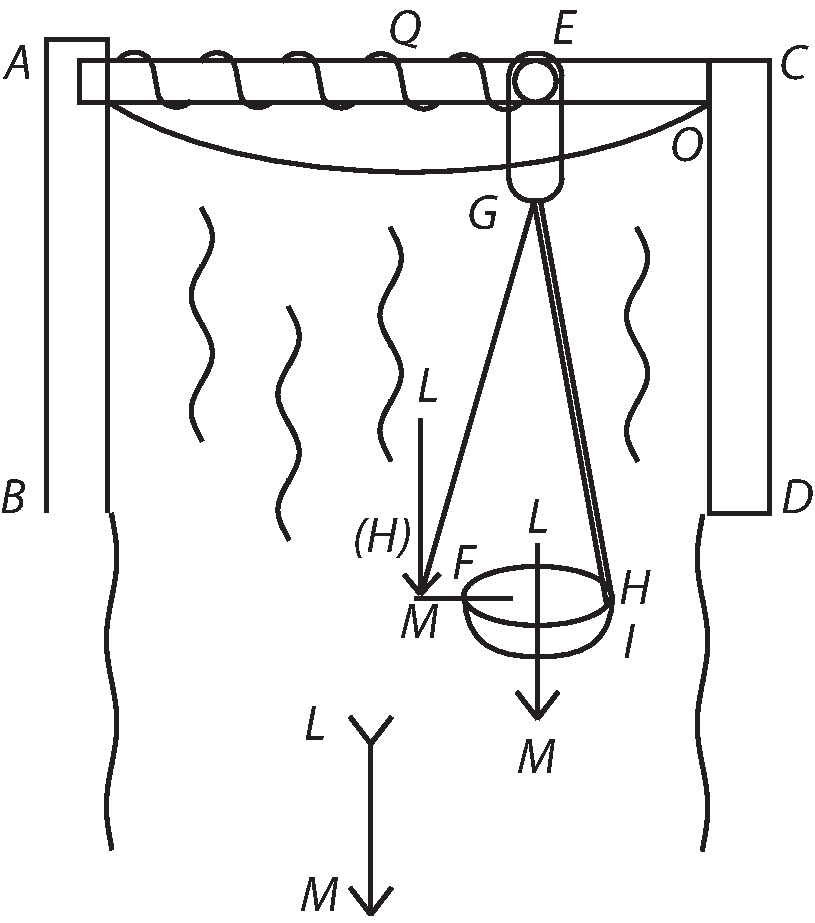
\includegraphics[width=0.6\textwidth]{images/38_87r1}
   \vspace{0.5ex}
   \\\textit{[Fig. 1]} \\
  \newpage
  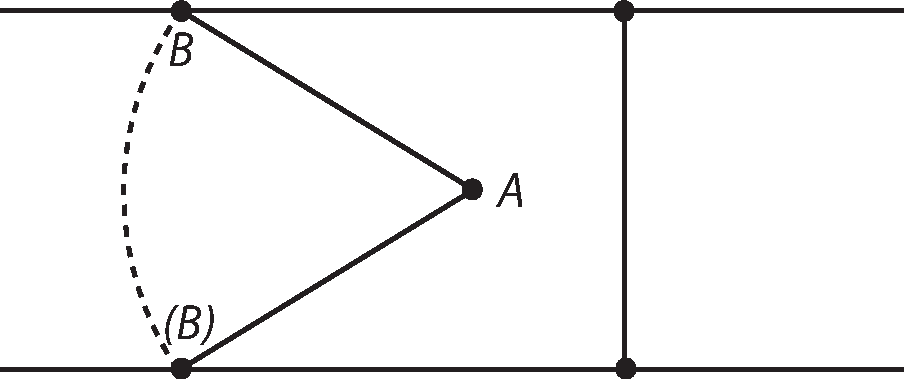
\includegraphics[width=0.6\textwidth]{images/38_87r2}
  \vspace{0.5ex}
   \\\textit{[Fig. 2]} \\
   \vspace{10mm}
  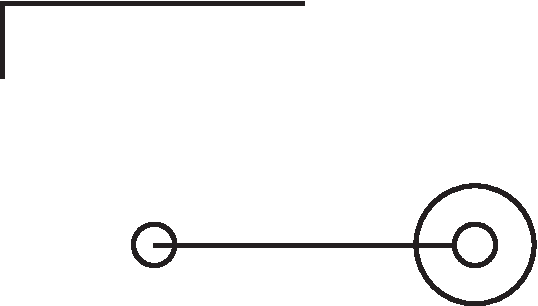
\includegraphics[width=0.4\textwidth]{images/38_87r3}
  \vspace{0.5ex}
   \\\textit{[Fig. 3]} \\
   \vspace{10mm}
  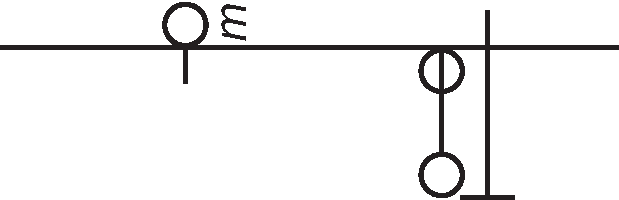
\includegraphics[width=0.4\textwidth]{images/38_87r4}
  \vspace{0.5ex}
   \\\textit{[Fig. 4]} \\
   \vspace{10mm}
  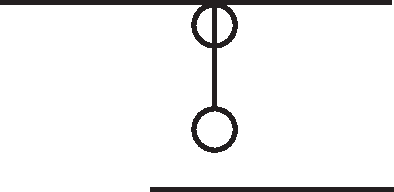
\includegraphics[width=0.4\textwidth]{images/38_87r5}
   \\\textit{[Fig. 5]}
 \end{center}